\documentclass[class=NCU_thesis, crop=false]{standalone}
\begin{document}

\chapter{背景知識以及文獻回顧}

\section{背景知識}
\subsection{大型語言模型的研究現況}

在自然語言處理(Natural Language Processing, NLP)~\cite{chowdhary2020natural}領域,大型語言模型的發展經歷了多個重要階段,這些階段的發展對於自然語言處理技術的進步和應用具有深遠的影響。以下是一些與自然語言處理相關的里程碑:

\begin{itemize}
    \item 早期階段:統計模型為當時主要的方法,但這些模型在處理複雜的語言時存在一定的局限性,特別是對於語境理解和生成的能力有限。

    \item 神經語言模型(Neural Language Model, NLM)~\cite{kim2016character}:神經語言模型的出現標誌著自然語言處理技術轉為使用類神經網路作為模型架構,但由於當時硬體計算能力和儲存空間的限制,這些模型的規模和性能十分有限。

    \item 變換器模型(Transformer Model)~\cite{wolf-etal-2020-transformers}:變換器模型的提出是自然語言處理領域的一個重要突破,它引入了自注意機制(Self-Attention),使模型能夠更好的捕捉序列中的長程依賴性,從而取得了顯著的性能提升。

    \item BERT(Bidirectional Encoder Representations from Transformers)~\cite{devlin2019bert}:BERT是一個雙向的Transformer模型,通過預訓練和微調,在多項自然語言處理任務上表現卓越。

    \item 大型語言模型(Large Language Model, LLM):在過去的幾年中,大型語言模型取得了巨大的進展,這些模型擅長理解和生成類人語言。
\end{itemize}


大型語言模型的發展是自然語言處理領域的一項重要突破,其基於大量文本數據(例如維基百科、網頁文本)進行無監督預訓練。透過預測下一個詞或填充遮罩的詞來學習語言結構,大型語言模型通常由多個變換器模型層疊加而成。這些變換器層不僅有助於模型學習不同的抽象詞彙,同時也借助自注意力機制,使其能夠有效地處理長文本序列。

最近,多模態模型(Large Multimodal Models, LMM)的出現使得現今的人工智慧技術不僅能夠處理文本資訊,還可以處理如圖像、音訊、影片等多種模式。這樣的多模態整合不僅能更全面地理解和生成內容,更大幅增加了人工智慧在現實生活中應用場景,如自動駕駛~\cite{cui2023survey}、藝術創作等~\cite{cai2023benchlmm}。而一些多模態模型也由於同時使用文本和圖像資料進行了聯合訓練,獲得了比大型語言模型更好的成效。

未來,大型語言模型的發展將面臨許多挑戰。其中包括模型的更好可解釋性,即如何讓模型的決策過程更加透明和可理解;更好的預訓練策略,以提高模型的效能和泛化能力;多模態整合的深入研究,以進一步拓展模型的應用範圍;以及更大模型規模的探索,以應對日益複雜的語言任務和多模態任務需求。

總之,大型語言模型的未來發展將在自然語言處理、多模態應用和人工智慧的其他領域中發揮重要作用,並將為人類社會帶來更加便利的服務與體驗。

\subsection{智慧機器與人工智慧物聯網的應用場景}

人工智慧物聯網(Artificial Intelligence of Things, AIOT)~\cite{9264235}技術目前已廣泛應用於許多領域,以下是一些典型的應用範例:

\begin{itemize}
    \item 工業4.0(Industry 4.0)~\cite{9695219}:工業領域是人工智慧物聯網技術應用的主要領域之一。機械臂在製造業中的應用越來越普遍。它們可以用於組裝、焊接、物料處理等高重複工作。人工智慧物聯網技術是智慧工廠實現生產過程的自動化和智能化的關鍵,這有助於提高生產效率並減少人力成本,從而提高了整個製造業的競爭力。

    \item 物流和倉儲:物流和倉儲管理是另一個智慧機器和人工智慧物聯網技術的重要應用場景。無人搬運車(Automated Guided Vehicle, AGV)~\cite{10021117}在物流和倉儲管理中扮演著關鍵角色。它們可以自動運送物品,根據預定路徑進行導航,不僅能夠實現倉庫內物品的快速移動和準確分配,同時也降低了人力成本,尤其是在大型倉庫和物流中心,對於智慧機器的需求更加顯著。

    \item 醫療保健~\cite{8893884}:智慧機器和人工智慧物聯網技術在醫療保健領域也有著重要的應用。手術機器人是其中一個典型的例子,它可以幫助外科醫生不受時間與地點的影響進行精確的手術操作,同時兼顧了手術的準確性、安全性與急迫性三個重要需求。此外,智慧機器人還可以應用於康復治療和輔助生活等方面,給予病患在進行康復訓練時能獲得更為良好的體驗。
\end{itemize}

綜上所述,人工智慧物聯網技術現今已廣泛應用於工業自動化、物流倉儲管理以及醫療保健等領域,不僅提高了生產效能,同時也改善了人們的生活品質和健康狀態。隨著技術的不斷發展和創新,人工智慧物聯網技術將繼續在各個領域發揮著重要作用,推動產業往智慧化、自動化的方向發展。

\subsection{3D列印技術的發展現況}
受惠於電腦輔助設計(Computer Aided Design, CAD)~\cite{sarcar2008computer}、電腦輔助製造(Computer-Aided Manufacturing, CAM)~\cite{elanchezhian2007computer}和電腦數值控制加工(Computer Numerical Control, CNC)~\cite{thyer2014computer}等技術的蓬勃發展。使快速成形技術~\cite{PHAM19981257}(Rapid Prototyping, RP)在現在的工業設計與製造的研究領域中,已越來越成熟。此技術時常用於快速生成零件模型的製造技術,它通過電腦控制,將材料進行堆疊加工,生成立體實品,因此又稱為積層製造技術(Additive Manufacturing, AM)~\cite{wong2012review},而3D列印(3 Dimensional Printing, , 3DP)~\cite{shahrubudin2019overview}則是此技術的一種具體應用。以下為3D列印技術的大致發展歷程:


\begin{itemize}
	\item 早期發展:在1981年,日本名古屋市工業研究所的小玉秀男提出了兩種利用光固化高分子的3D列印方法。隨後,美國3D系統公司的Chuck Hull發展了一套快速成形系統,稱為立體快速成形(Stereolithography, SLA),利用紫外線雷射來固化光聚合物。

	\item 商業化時期:1986年,3D系統公司在美國通過了第一個快速成形設備的專利,並在1988年開發出第一台商業化的快速成形系統。1989年,美國麻省理工學院申請了第一個3D列印的專利技術。早期的技術專利主要掌握在大型快速成形系統公司手中,但直到2010年,這些專利陸續到期,3D列印的應用開始蓬勃發展。

	\item 應用發展時期:從2010年開始,3D列印的市場產值逐年提升,應用層面也愈加廣泛,現今的3D列印技術已被廣泛應用於建築、工業設計、汽車、航太、醫療生技、服飾、飾品、地理資訊和食品等產業。一些劃時代的成品包括3D列印的房屋~\cite{hager20163d}、無人機~\cite{moon2014application}、汽車~\cite{chinthavali20163d}、人工血管~\cite{papaioannou20193d}和各式食品~\cite{liu20173d}都已在近年陸續問世。

\end{itemize}
3D列印作為快速成形技術技術的一種具體應用,經歷了從早期發展到商業化時期再到應用發展時期的演進過程。從1980年代的技術創新到2010年後的市場爆發,3D列印直到現在依然在不斷擴展應用範圍,隨著技術的不斷發展,3D列印將持續在各個領域中發揮重要作用,為各行各業帶來更多創新與可能性。

\section{文獻回顧}
\subsection{大型語言模型及其在程式碼生成與機器控制上的應用}

Vaithilingam等人~\cite{vaithilingam2022expectation}為了探討大型語言模型作為程式碼生成工具的可用性,招募了24名擁有不同程式設計經驗的參與者,使用Copilot,這個基於大型語言模型的程式碼生成工具,執行一系列不同難度的程式設計任務,而研究人員則從旁紀錄每個餐與者的操作、用時與使用Copilot的心得。而研究發現,大多數參與者都喜歡在進行程式設計時使用 Copilot,因為它能夠提供一個有用的起點,讓使用者能節省許多思考與搜索的時間,能直接使用Copilot給予的程式為基礎繼續進行修改,然而,有些參與者也同時在理解、編輯 Copilot生成的程式碼片段時遇到了困難,導致拖延了任務完成的進度。此研究最後總結了一些關於這類程式碼生成工具的改進方向,鼓勵使用者不應簡單的將Copilot視為一個能一步到位程式碼產生工具,而應該為理解和驗證生成的程式碼,進而去探索更多解決方案和任務解方。

Sai等人~\cite{vemprala2023chatgpt}探討了ChatGPT在機器人應用中的實驗研究,並提出了一種策略,結合了提示工程的設計原則和機器控制函式,使ChatGPT能透過與人對話、解析XML標記以及合成程式碼,完成機器人領域的一系列任務,其中例如導航、控制無人機與機械臂,研究重點在於不同的對話策略,在執行各種類型的機器人任務時,是否有成效上的差別。其中還介紹了一個名為PromptCraft的開源研究工具,其中包含一個平台,研究人員可以共同上傳並投票選出最優的對話策略,以及一個集成了ChatGPT的機器人模擬器,讓使用者更容易進行ChatGPT與機器人之間的相關研究。

Liang等人~\cite{10160591}的研究提出了名為「程式即為策略」(Code as Policies)的方法,使用大型語言模型直接生成可以作為控制機器人策略的程式。實驗結果表明,使用大型語言模型生成的程式碼,在某些實驗中的確可以成功地控制機器人執行各種指令,包括某些新的、且沒見過的指令,不過隨著任務難度的複雜化,實驗中隨之降低的準確率也展示出了,現今大型語言模型在語意推理和空間幾何推理領域的發揮是有限的。不過,這篇論文提出的方法仍為機器人控制領域帶來了新的思路,也展示了機器控制與大型語言模型結合後的技術前景。


由文獻可以得知,大型語言模型在機器控制領域與其他眾多領域擁有許多可能性。

\subsection{運動學研究與機器人控制}

機器人與問動學的研究早已行之有年,以下使用~\cite{kucuk2006robot}提供的定義對本問題做一個簡單解釋:
\begin{itemize}
	\item 順向運動學 (Forward Kinematics): 順向運動學是一個關鍵概念,它使我們能透過關節角度計算出機械臂末端的位置。這對於控制機械手臂非常重要,因為它使我們能透過馬達角度確定機械臂的每個關節點的空間座標。

	\item 逆向運動學 (Inverse Kinematics): 逆向運動學是正向運動學的反向問題。它試圖根據機械臂末端的位置,計算出每個關節應該轉動的角度。這是一個更困難的問題,因為它涉及到解方程組或使用數值方法來找到關節角度。逆向運動學在機械手臂的路徑規劃和避障中至關重要。
\end{itemize}

在順向運動學中,Denavit-Hartenberg為最常用的計算方式。此方法使用四個參數來計算力臂頂點座標: 
\begin{itemize}
    \item $a_{i}$:力臂長度(Link length),指在第$i$個力臂上,從第$i$個關節的旋轉軸到第$i+1$個關節的旋轉軸之間的距離,此參數沿著第$i$個力臂的$Z_{i}$軸測量。
    \item $\alpha_{i}$:扭轉角(Twist Angle),兩個力臂的連接處稱為節點,指從第$i$個節點到第$i+1$個節點之間的扭轉角度,此參數沿著第$i$個節點$X_{i}$軸測量。
    \item $d_{i}$:節點偏移(Link offset),指從第$i$個節點到第$i+1$個節點之間的距離,此參數通常是變量。
    \item $\theta_{i}$:節點角度(Joint angle),指第$i$個旋轉軸的旋轉角度,此參數通常是變量。
\end{itemize}
每個關節都使用一個獨立座標系來決定這些參數。

\begin{figure}[htbp]
    \centering
    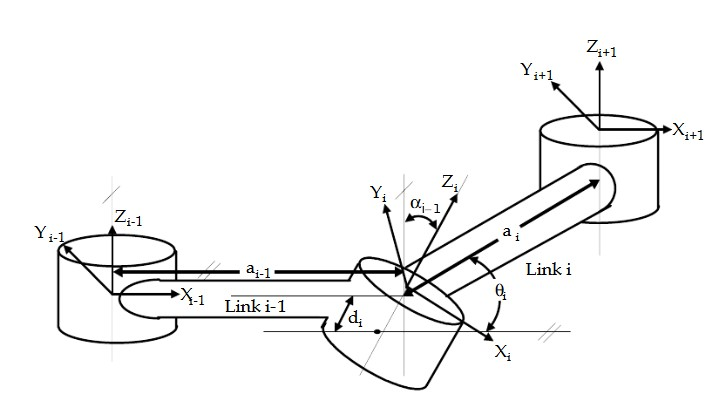
\includegraphics[width=0.9\textwidth]{figures/Coordinate frame assignment for a general manipulator.jpg}
\caption{順向運動學示例圖}
\end{figure}

如上圖所示,沿$X_{i-1}$測得的$Z_{i-1}$到$Z_{i}$的距離記$a_{i-1}$,沿$X_{i}$測得的$Z_{i-1}$和$Z_{i}$之間的角度為$\alpha_{i-1}$,沿$Z_{i}$測得的$X_{i-1}$到$X_{i}$的距離記$d_{i}$,沿$Z_{i}$測得的$X_{i-1}$到$X_{i}$的角度記$\theta_{i}$。\\
如此可求得變換矩陣${ }_{\mathrm{i}}^{\mathrm{i}-1} \mathrm{~T}$:

\begin{small}
\begin{align}
\nonumber
& { }_{\mathrm{i}}^{\mathrm{i}-1} \mathrm{~T}=\mathrm{R}_{\mathrm{x}}\left(\alpha_{\mathrm{i}-1}\right) \mathrm{D}_{\mathrm{x}}\left(\mathrm{a}_{\mathrm{i}-1}\right) \mathrm{R}_{\mathrm{z}}\left(\theta_{\mathrm{i}}\right) \mathrm{Q}_{\mathrm{i}}\left(\mathrm{d}_{\mathrm{i}}\right) \\
\nonumber
& =
\left[\begin{array}{cccc}
1 & 0 & 0 & 0 \\
0 & \cos \alpha_{i-1} & -\sin \alpha_{i-1} & 0 \\
0 & \sin \alpha_{i-1} & \cos \alpha_{i-1} & 0 \\
0 & 0 & 0 & 1
\end{array}\right]
\nonumber
\left[\begin{array}{cccc}
1 & 0 & 0 & a_{i-1} \\
0 & 1 & 0 & 0 \\
0 & 0 & 1 & 0 \\
0 & 0 & 0 & 1
\end{array}\right]
\nonumber
\left[\begin{array}{cccc}
\cos \theta_{i} & -\sin \theta_{i} & 0 & 0 \\
\sin \theta_{i} & -\cos \theta_{i} & 0 & 0 \\
0 & 0 & 1 & 0\\
0 & 0 & 0 & 1
\end{array}\right]
\nonumber
\left[\begin{array}{cccc}
1 & 0 & 0 & 0 \\
0 & 1 & 0 & 0 \\
0 & 0 & 1 & d_{i} \\
0 & 0 & 0 & 1
\end{array}\right]\\
\nonumber
& =\left[\begin{array}{cccc}
\cos \theta_{i} & -\sin \theta_{i} & 0 & a_{i-1} \\
\sin \theta_{i} \cos \alpha_{i-1} & \cos \theta_{i} \cos \alpha_{i-1} & -\sin \alpha_{i-1} & -\sin \alpha_{i-1} d_{i} \\
\sin \theta_{i} \sin \alpha_{i-1} & \cos \theta_{i} \sin \alpha_{i-1} & \cos \alpha_{i-1} & \cos \alpha_{i-1} d_{i} \\
0 & 0 & 0 & 1
\end{array}\right] \\
\nonumber
&\end{align}
\end{small}

而逆向運動學問題,實驗中使用了幾何求解(Geometric solution approach),與策略梯度方法(Policy-Gradient solution approach)~\cite{dauce2010inverse}來開發機械臂的逆向控制。\\

幾何求解方法的原理是將機械手臂的空間幾何問題分解為多個平面幾何問題,適用於機械結構較為簡單的機器人,如下圖所示:

\begin{figure}[htbp]
    \centering
    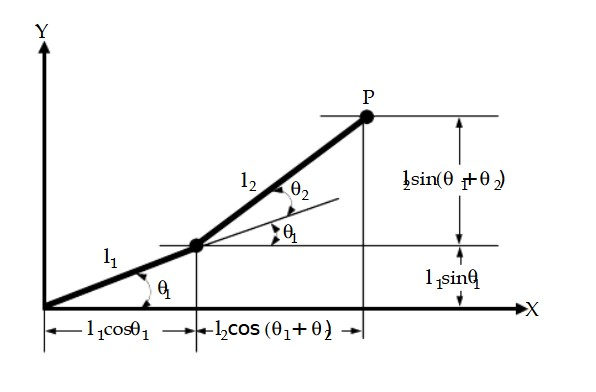
\includegraphics[width=0.9\textwidth]{figures/IK.jpg}
\caption{幾何求解逆向運動學示例圖}
\end{figure}

可由以下算式機算頂點$P$的分量($P_{x}$, $P_{y}$)。
$$
\begin{aligned}
& p_{x}=l_1 \cos \theta_1+l_2 \cos \theta_{12} \\
& p_{y}=l_1 \sin \theta_1+l_2 \sin \theta_{12}
\end{aligned}
$$
由於,$\cos \theta_{12}=\cos \theta_{1} \cos \theta_{2}-\sin \theta_{1} \sin \theta_{2}$,$
\sin \theta_{12}=\sin \theta_{1} \cos \theta_{2}-\cos \theta_{1} \sin \theta_{2}$,所以可得:

$$
\begin{small}
\begin{aligned}
& p_{x}^2=l_1^2 \cos^2 \theta_1+l_2^2 \cos^2 \theta_{12}+2 l_1 l_2 \cos \theta_1 \cos \theta_{12} \\
& p_{y}^2=l_1^2 \sin^2 \theta_1 + l_2^2 \sin^2 \theta_{12}+2 l1_2 \sin \theta_1 \sin \theta_{12} \\
& p_{x}^2+p_{y}^2=l_1^2\left(\cos^2 \theta_1+\sin^2 \theta_1\right)+l_2^2\left(\cos^2 \theta_{12}+\sin^2 \theta_{12}\right)+2l_1 l_2\left(\cos \theta_1 \cos \theta_{12}+\sin \theta_1 \sin \theta_{12}\right)
\end{aligned}
\end{small}
$$

由於$\cos^2 \theta_{i}+\sin^2 \theta_{i}=1$,故可將上式化簡為:

$$
\begin{small}
\begin{aligned}
& p_{x}^2+p_{y}^2=l_1^2+l_2^2+2l_1 l_2\left(c \theta_1\left[\cos \theta_1 \cos \theta_2-\sin \theta_1 \sin \theta_2\right]+\sin \theta_1\left[\sin \theta_1 \cos \theta_2+\cos \theta_1 \sin \theta_2\right]\right) \\
& p_{x}^2+p_y^2=l_1^2+l_2^2+2l_1 l_2\left(\cos^2 \theta_1 \cos \theta_2-\cos \theta_1 \sin \theta_1 \sin \theta_2+\sin^2 \theta_1 \cos \theta_2+\cos \theta_1 \sin \theta_1 \sin \theta_2\right) \\
& p_{x}^2+p_y^2=l_1^2+l_2^2+2l_1 l_2\left(\cos \theta_2\left[\cos^2 \theta_1+\sin^2 \theta_1\right]\right) \\
& p_{x}^2+p_{y}^2=l_1^2+l_2^2+2l_1 l_2 \cos \theta_2
\end{aligned}
\end{small}
$$

由移項後得:

$$
\begin{aligned}
& \cos \theta_2=\frac{p_{x}^2+p_{y}^2-l_1^2-l_2^2}{2l_1 l_2} \\
& \sin \theta_2= \pm \sqrt{1-\left(\frac{p_{x}^2+p_{y}^2-l_1^2-l_2^2}{2l_1 l_2}\right)^2} \\
& \theta_2=A \tan 2\left( \pm \sqrt{1-\left(\frac{p_{x}^2+p_{y}^2-l_1^2-l_2^2}{2l_1 l_2}\right)^2}, \frac{p_{x}^2+p_{y}^2-l_1^2-l_2^2}{2l_1 l_2}\right)
\end{aligned}
$$

繼續利用$\theta_2$求解$\theta_1$:
將$p_{x}=l_1 \cos \theta_1+l_2 \cos \theta_{12}$等號兩邊同乘$\cos \theta_1$
將$p_{y}=l_1 \sin \theta_1+l_2 \sin \theta_{12}$等號兩邊同乘$\sin \theta_1$得:
$$
\begin{small}
\begin{aligned}
& \cos \theta_1 p_{x}=l_1 \cos^2 \theta_1+l_2 \cos^2 \theta_1 \cos \theta_2-l_2 \cos \theta_1 \sin \theta_1 \sin \theta_2 \\
& \sin p_{y}=l_1 \sin^2 \theta_1+l_2 \sin^2 \theta_{1} \cos \theta_2+l_2 \sin \theta_1 \cos \theta_1 \sin \theta_2 \\
& \cos \theta_1 p_{x}+\sin \theta_1 p_{y}=l_1\left(\cos^2 \theta_1+\sin^2 \theta_1\right)+l_2 \theta_2\left(\cos \theta_1+\sin^2 \theta_1\right)
\end{aligned}
\end{small}
$$
可化簡為:
$$
\cos \theta_1 p_{x}+\sin \theta_1 p_{y}=l_1+l_2 \cos \theta_2
$$

將$p_{x}=l_1 \cos \theta_1+l_2 \cos \theta_{12}$等號兩邊同乘$-\sin \theta_1$
將$p_{y}=l_1 \sin \theta_1+l_2 \sin \theta_{12}$等號兩邊同乘$\cos \theta_1$得:
$$
\begin{small}
\begin{aligned}
& -\sin \theta_1 p_{x}=-l_1 \sin \theta_1 \cos \theta_1-l_2 \sin \theta_1 \cos \theta_1 \cos \theta_2+l_1 \sin^2 \theta_1 \sin \theta_2 \\
& \cos \theta_1 p_{y}=l_1 \sin \theta_1 \cos \theta_1+l_2 \cos \theta_1 \sin \theta_1 \cos \theta_2+l_2 \cos^2 \theta_1 \sin \theta_2 \\
& -\sin \theta_1 p_{x}+\cos \theta_1 p_{y}=l_2 \sin \theta_2\left(\cos^2 \theta_1+\sin \theta_1\right)
\end{aligned}
\end{small}
$$
可化簡為:
$$
-\sin \theta_1 p_{x} + \cos \theta_1 p_{y} = l_2 \sin \theta_2
$$

最後,將$\cos \theta_1 p_{x}+\sin \theta_1 p_{y}=l_1+l_2 \cos \theta_2$等號兩邊同乘$P_x$,$-\sin \theta_1 p_{x} + \cos \theta_1 p_{y} = l_2 \sin \theta_2$等號兩邊同乘$P_y$,得:

$$
\begin{aligned}
& \cos \theta_1 p_{x}^2 + \sin \theta_1 p_x p_y = p_x \left(l_1 + l_2 \cos \theta_2 \right) \\
& - \sin \theta_1 p_x p_y + \cos \theta_1 p_{y}^2 = p_y l_2 \sin \theta_2 \\
& \cos \left(p_{x}^2+p_{y}^2 \right) = p_x \left(l_1+l_2 \cos \theta_2 \right) - p_y l_2 \sin \theta_2
\end{aligned}
$$
可求出$\theta_1$:
$$
\begin{small}
\begin{aligned}
& \cos \theta_1= \frac{p_x \left(l_1+l_2 \cos \theta_2 \right)+p_y l_2 \sin \theta_2}{p_x^2 + p_y^2} \\
& \sin \theta_1= \pm \sqrt{1-\left(\frac{p_{x} \left(l_1 + l_2 \cos \theta_2 \right)+p_y l_2 \sin \theta_2}{p_x^2 = p_y^2}\right)^2} \\
& \theta_1=A \tan 2\left( \pm \sqrt{1-\left(\frac{p_{x}\left(l_1+l_2 \cos \theta_2\right)+p_{y} l_2 \sin \theta_2}{p_{x}^2+p_{y}^2}\right)^2}, \frac{p_{x}\left(l_1+l_2 \cos \theta_2\right)+p_{y} l_2 \sin \theta_2}{p_{x}^2+p_{y}^2}\right)
\end{aligned}
\end{small}
$$

以上為使用幾何求解逆向運動學的簡易範例,可以看出使用此方法求解需要繁瑣的計算。 \\

以下介紹使用策略梯度方法求解逆向運動學的計算方式:

\subsection{3D列印應用於機器人製作的相關文獻}
引用carbon design的相關論文並進一步討論(用於設計3D模型)

\end{document}